%!TEX program = xelatex
\documentclass[a4paper,UTF8]{ctexart}
\usepackage[unicode=true,colorlinks,urlcolor=blue,linkcolor=blue,bookmarksnumbered=true]{hyperref}
\usepackage{latexsym,amssymb,amsmath,amsbsy,amsopn,amstext,amsthm,amsxtra,color,multicol,bm,calc,ifpdf}
\usepackage{graphicx}
\usepackage{diagbox}   % 绘制表格斜线
\usepackage{enumerate}
\usepackage{epstopdf}
\usepackage{fancyhdr}
\usepackage{subfigure}
\usepackage{listings}
\usepackage{multirow}
\usepackage{makeidx}
\usepackage{xcolor} 
\usepackage{algorithm}    % format of the algorithm
\usepackage{algorithmic}    % format of the algorithm
\usepackage{fontspec}                            % 建立索引宏包
\graphicspath{{figures/}}  % 设置图片搜索路径
\theoremstyle{plain} \newtheorem{theorem}{定理}[section]
\theoremstyle{plain} \newtheorem{definition}{定义}[section]
\theoremstyle{plain} \newtheorem{lemma}{引理}[section]
\theoremstyle{plain} \newtheorem{proposition}{命题}[section]
\theoremstyle{plain} \newtheorem{example}{例}[section]
\theoremstyle{plain} \newtheorem{remark}{注}[section]
\theoremstyle{plain} \newtheorem{corollary}{推论}[section]
\newfontfamily\courier{Courier New}
\lstset{linewidth=1.1\textwidth,
        numbers=left, %设置行号位置 
        basicstyle=\small\courier,
        numberstyle=\tiny\courier, %设置行号大小  
        keywordstyle=\color{blue}\courier, %设置关键字颜色  
        %identifierstyle=\bf,
        commentstyle=\it\color[cmyk]{1,0,1,0}\courier, %设置注释颜色 
        stringstyle=\it\color[RGB]{128,0,0}\courier,
        %framexleftmargin=10mm,
        frame=single, %设置边框格式  
        backgroundcolor=\color[RGB]{245,245,244},
        %escapeinside=``, %逃逸字符(1左面的键),用于显示中文  
        breaklines, %自动折行  
        extendedchars=false, %解决代码跨页时,章节标题,页眉等汉字不显示的问题  
        xleftmargin=2em,xrightmargin=2em, aboveskip=1em, %设置边距  
        tabsize=4, %设置tab空格数  
        showspaces=false %不显示空格  
        basicstyle=\small\courier
       }  
\newenvironment{mysolution}{{\color{blue} 解}: }{{\color{magenta}\qed}}
\newcommand\diff{\,{\mathrm d}} %定义微分d
\newcommand{\p}[3]{\frac{\partial^{#1}#2}{\partial{#3}^{#1}}}  %定义求偏导算子
\newcommand{\ucite}[1]{\textsuperscript{\cite{#1}}}  %参考文献引用:上标用\ucite{ },文中用\cite{ }

\begin{document}
\title{

\includegraphics[width=0.65\textwidth]{onepiece.pdf}\\
\vspace{2em}
\textbf{MCMC 方法学习笔记}}
\author{\emph{李向阳} \quad {\color{blue} d1142845997@gmail.com} }
\date{}


\maketitle
\thispagestyle{empty}

\newpage


\tableofcontents

\newpage

\section{引入}
本次我们暂不介绍具体的机器学习算法, 而是讲述一下 Mento Carlo Markov Chain (简称 MCMC) 方法. 所谓 MCMC 方法, 其实是一种采样的方法. 采样问题指的是给定一个特定的概率分布$p(z)$, 得到一批符合这个概率分布的样本点. 那么采样方法有什么应用呢?

我们对蒙特卡罗方法已经很熟悉了, 高中就接触过如何通过撒豆子等随机模拟方法计算圆周率或者定积分等, 记得当时也用计算器产生随机数模拟了一下, 现在到了大学直接用计算机编程就可以模拟了. 其实这就算采样方法的一个应用.

以计算积分为例, 采样方法可以用在贝叶斯估计中. 在完整的贝叶斯估计中, 我们需要写出完整的后验概率的函数公式, 而不是只根据 MLE 或者 MAP 求最大值, 即
\begin{equation*}
p(\bm{\theta} | X) = \frac{p(X | \bm{\theta}) p(\bm{\theta})}{p(X)} = \frac{p(X | \bm{\theta}) p(\bm{\theta})}{\displaystyle \int p(X | \bm{\theta}) p(\bm{\theta}) \diff \bm{\theta}}
\end{equation*}

其中$p(X | \bm{\theta})$是似然函数, $p(\bm{\theta})$是先验概率密度, 最关键的是需要计算积分$\displaystyle \int p(X | \bm{\theta}) p(\bm{\theta}) \diff \bm{\theta}$, 我们可以把问题一般化如下:

假设$Z$是一个连续随机变量(离散的情况类似), 其概率密度函数为$p(z)$, 现在要计算函数$f(z)$的期望值, 即
\begin{equation*}
\mathbb{E}[f(z)] = \int f(z) p(z) \diff z
\end{equation*}

如果我们能根据$p(z)$采样出一堆点$z^{(0)}, z^{(1)}, \cdots, z^{(n)}$, 那么我们用这些点代入函数求均值, 随着采样点的增多, 得到的结果就会越来越逼近理论结果:
\begin{equation*}
\mathbb{E}[f(z)] = \lim_{N \rightarrow \infty} \frac{1}{N} \sum_{t=1}^{N} f(z^{(t)})
\end{equation*}

所以采样方法还是很有用的(虽然处理这个积分还有变分贝叶斯方法), 当然还有很多其他用处, 下面就来稍微介绍一下.


\section{马尔科夫链}
之前我们介绍 PageRank 算法时, 稍微提及了马尔科夫过程. 其实, 马尔科夫链和马尔科夫过程应该是我们上随机过程课程的时候讲的, 无奈当时课时短所以没讲到. 所以, 关于马尔科夫链等东西可参考具体的随机过程的课本. 这里不太严谨的说明一下.

\subsection{随机矩阵}
我们这里讲的随机矩阵, 在英语中是 Stochastic Matrix (而不是 Random Matrix, 每个元素都是随机数), 它是用来描述一个马尔科夫链的转变的矩阵, 又称概率矩阵、 转移矩阵. 它的每一项都是一个表示概率的非负实数.

在不同的方向中, 有几种不同的类型或者说定义的随机矩阵:
\begin{enumerate}[(1)]
\item 行(右)随机矩阵是实方阵, 其每一行元素之和为$1$.

\item 列(左)随机方阵是实方阵, 其每一列元素之和为$1$.

\item 双随机矩阵是非负实数矩阵, 其每行元素和每列元素之和均为$1$.
\end{enumerate}

设$A$是一个行随机矩阵, $\bm{e}$是元素全为$1$的列向量, 即$\bm{e} = (1, 1, \cdots, 1)^{T}$, 我们知道因为矩阵$A$的每行元素之和为$1$, 所以它有一个特征值为$1$, 且相应的特征向量为$\bm{e}$, 即有
\begin{equation*}
A \bm{e} = \bm{e}
\end{equation*}

同理, 若设$A$是一个列随机矩阵, $\bm{e}$是元素全为$1$的行向量, 即$\bm{e} = (1, 1, \cdots, 1)$, 由于$A^{T}$为行随机矩阵, 因此可得
\begin{equation*}
A^{T} \bm{e}^{T} = \bm{e}^{T} \Rightarrow \bm{e} A = \bm{e}
\end{equation*}

当然, 这也可以由$A$的每列元素之和均为$1$看出来.

\subsection{马尔科夫链的性质}
什么是马尔科夫链呢? 这里我们不给出严谨的定义, 因为说过了可在各种随机过程课本里找到, 只给出一个简单的例子. 

想象一个国家, 其城市人口和农村人口会每年发生一次迁移, 并且假设迁移概率是固定的, 每年城市迁农村的概率是$3 \%$, 农村迁城市的概率是$5 \%$, 也就是说概率转移矩阵为
$$
P = 
\begin{bmatrix}
0.97 & 0.03 \\ 
0.05 & 0.95
\end{bmatrix}
$$

如果某一年城市和农村的人口分别是2000和14000, 那么下一年的人口分布是怎么样的呢? 我们可以用如下的矩阵计算表示
$$
[2000 \quad 14000] \cdot 
\begin{bmatrix}
0.97 & 0.03 \\ 
0.05 & 0.95
\end{bmatrix}
= [2640 \quad 13360]
$$

而作为一个个体, 其实是在不同的状态(农村或城市)之间跳转的, 比如$t=1$时是农村人, $t=2$时是城市人. 马尔可夫链就是生成这样一段状态序列的随机过程, 其中城市和农村互相流动的矩阵, 叫做迁移矩阵, 也就是概率转移矩阵. 马尔可夫链的这个随机过程满足马尔科夫性质, 也就是某一个状态的值只跟前一个状态相关, 用公式表示就是
\begin{equation*}
P(X_n = x | X_{n-1}, \cdots, X_0) = P(X_n = x | X_{n-1})
\end{equation*}

每次计算下一年的人口分布情况, 都可以这样迭代计算. 当状态迭代到一定程度之后, 我们会发现, 城市和农村的人数趋于一个稳定值, 其中城市人数是$10000$, 农村人数是$6000$. 而且我们用任意一个总人口为16000的状态作为初始状态, 最后的结果都是这个. 对于个体来说, 这就是个体会留在农村还是城市的概率分布, 也就是留在城市和农村的概率比为5:3, 或者说概率分布为$(5/8, 3/8)$, 这个分布也叫马尔可夫链的平稳分布.

简单起见, 这里不加证明的简单描述下马尔科夫链的收敛性质(暂时不管前提条件):
\begin{enumerate}[(1)]
\item 马尔可夫链模型收敛于平稳分布$\bm{\pi}$, 满足对于转移矩阵$P$, $\bm{\pi}$是方程$\bm{\pi} P = \bm{\pi}$的唯一解, 其中$\bm{\pi}$为一个行向量, 其分量就是平稳分布在各个取值上对应的概率, 即$\bm{\pi} = [\pi(0), \pi(1), \cdots, \pi(i), \cdots], \sum_{i} \pi(i) = 1$

\item 转移矩阵$P$本身经过反复迭代之后也要收敛(每列结果相同), 才能满足平稳分布的要求, 即
$$
\lim_{n \rightarrow \infty} P^{n} = 
\begin{bmatrix}
\pi(0) & \pi(1) & \cdots & \pi(i) & \cdots \\ 
\pi(0) & \pi(1) & \cdots & \pi(i) & \cdots \\ 
\pi(0) & \pi(1) & \cdots & \pi(i) & \cdots \\ 
\cdots & \cdots & \cdots & \cdots & \cdots 
\end{bmatrix}
$$

\end{enumerate}



\section{MCMC 采样}
\subsection{Metropolis-Hastings 算法}
既然马尔科夫链可以收敛于一个平稳分布, 如果这个分布恰好是我们需要采样的分布$p(x)$, 那么当马尔科夫链在第$n$步收敛之后, 其后续不断生成的序列$X_{n}, X_{n+1}, \cdots$就可以当做是采样的样本. 这就是 MCMC 方法的基本思想. 那么如何找到符合条件的迁移矩阵$P$, 来得到目标分布$p(x)$的采样呢?

利用细致平稳条件可以解决这个问题, 该定理陈述如下:
\begin{theorem}
\textbf{细致平稳条件}: 如果非周期马氏链的转移概率矩阵$P$和某个分布$\bm{\pi}(x)$满足
\begin{equation*}
\pi(i) P_{ij} = \pi(j) P_{ji}, \quad \forall \quad i, j 
\end{equation*}

则$\bm{\pi}(x)$就是该马氏链的平稳分布.

\end{theorem}

假设我们有一个初始的转移矩阵$Q$, 其元素$q(i, j)$表示从状态$i$转移到状态$j$的概率, 也可以写为$q(j | i)$或$q(i \rightarrow j)$. 显然, 通常情况下
\begin{equation*}
p(i) q(i,j) \neq p(j) q(j,i)
\end{equation*}

也就是细致平稳条件不成立, 所以$p(x)$不太可能是这个马氏链的平稳分布. 那我们可否对马氏链做一个改造, 使得细致平稳条件成立呢? 比如, 可以引入$\alpha(i,j)$, 使得
\begin{equation*}
p(i) q(i,j) \alpha(i,j) = p(j) q(j,i) \alpha(j,i)
\end{equation*}

取什么样的$\alpha(i,j)$能使上式成立呢? 最简单的, 按照对称性, 可以取
\begin{equation*}
\alpha(i,j) = p(j) q(j,i), \quad \alpha(j,i) = p(i) q(i,j)
\end{equation*}

这样就有
\begin{equation*}
p(i) \underbrace{q(i,j) \alpha(i,j)}_{Q'(i,j)} = p(j) \underbrace{q(j,i) \alpha(j,i)}_{Q'(j,i)}
\end{equation*}

于是我们把原来具有转移矩阵$Q$的一个普通的马氏链, 改造为了具有转移矩阵$Q'$的马氏链, 而$Q'$恰好满足细致平稳条件, 因此马氏链$Q'$的平稳分布就是$p(x)$.

在改造$Q$的过程中引入的$\alpha(i,j)$称为接受率, 可以理解为在原来的马氏链上, 从状态$i$以$q(i,j)$的概率跳转到状态$j$的时候, 我们以$\alpha(i,j)$的概率接受这个转移, 于是得到新的马氏链$Q'$的转移概率为$q(i,j) \alpha(i,j)$.

假设我们的初始化转移矩阵为$Q$, 其元素为$q(i,j)$, 把上面的过程整理一下便得到了如下用于采样概率分布$p(x)$的算法.

\begin{algorithm}[htb]
\caption{算法: 基本 MCMC 采样算法}

\begin{enumerate}[1.]
\item 初始化马氏链初始状态$X_0 = x_0$和迁移矩阵$Q$ 

\item 对$t = 0,1,2,\cdots$, 循环以下过程进行采样
\begin{itemize}
    \item  根据当前时刻的状态$X_t = x_t$, 采样$y \sim q(x | x_t)$

    \item 计算接受率$\alpha(x_t, y) = p(y) q(x_t | y)$

    \item 从均匀分布随机抽样一个值$u$, 如果小于$\alpha(x_t, y)$, 则接受转移, 即令$X_{t+1} = y$, 否则令$X_{t+1} = x_t$
\end{itemize}
\end{enumerate}

\end{algorithm}

以上过程中$p(x), q(x | y)$均是离散情形, 事实上即便是这两个分布是连续的, 算法仍然有效, 即它可适用于一般的连续概率分布$p(x)$, 此时$q(x | y)$是任意一个连续二元概率分布对应的条件分布.

以上的基本 MCMC 采样算法已经能够工作了, 不过它有一个小问题, 马氏链$Q$在转移的过程中的接受率$\alpha(i,j)$可能偏小, 这样在采样过程中马氏链容易原地踏步, 拒绝大量的跳转, 这使得马氏链遍历所有的状态空间要花费太长的时间, 收敛到平稳分布的速度太慢. 那有没有办法提升一下接受率呢?

假设$\alpha(i,j) = 0.1, \alpha(j,i) = 0.2$满足细致平稳条件, 即有
\begin{equation*}
p(i) q(i,j) \times 0.1 = p(j) q(j,i) \times 0.2
\end{equation*}

上式两部扩大$5$倍, 即为
\begin{equation*}
p(i) q(i,j) \times 0.5 = p(j) q(j,i) \times 1
\end{equation*}

看, 我们提高了接受率, 而细致平稳条件并没有打破! 这启发我们可以把细致平稳条件中的$\alpha(i,j), \alpha(j,i)$同比例放大, 使得两数中最大的一个放大到$1$, 这样就提高了采样中的跳转接受率, 所以我们可以取
\begin{equation*}
\alpha(i,j) = \min \left\{ \frac{p(j) q(j,i)}{p(i) q(i,j)}, 1 \right\}
\end{equation*}

其实这一步目前并没有看懂(泪). 总之, 经过对上述 MCMC 采样算法中接受率的微小改动, 我们便得到了很多课本里最常见的 Metropolis-Hastings 算法.

\begin{algorithm}[htb]
\caption{算法: Metropolis-Hastings 算法}

\begin{enumerate}[1.]
\item 初始化马氏链初始状态$X_0 = x_0$和迁移矩阵$Q$ 

\item 对$t = 0,1,2,\cdots$, 循环以下过程进行采样
\begin{itemize}
    \item  根据当前时刻的状态$X_t = x_t$, 采样$y \sim q(x | x_t)$

    \item 计算接受率$\alpha(x_t, y) = \min \left\{ \dfrac{p(y) q(x_t | y)}{p(x_t) q(y | x_t)}, 1 \right\}$

    \item 从均匀分布随机抽样一个值$u$, 如果小于$\alpha(x_t, y)$, 则接受转移, 即令$X_{t+1} = y$, 否则令$X_{t+1} = x_t$
\end{itemize}
\end{enumerate}

\end{algorithm}

我们可以模拟一下 beta 分布, 其概率密度为
\begin{equation*}
p(x) = \frac{\Gamma(\alpha + \beta)}{\Gamma(\alpha) \Gamma(\beta)} x^{\alpha - 1} (1 - x)^{\beta - 1}
\end{equation*}

Python 代码如下
\begin{lstlisting}[language = python]
# -*- coding: utf-8 -*-

import random
import numpy as np
import pylab as pl
import scipy.special as ss

# 完整的beta分布概率密度函数
def beta(a, b, i):
    e1 = ss.gamma(a + b)
    e2 = ss.gamma(a)
    e3 = ss.gamma(b)
    e4 = i ** (a - 1)
    e5 = (1 - i) ** (b - 1)
    return (e1 / (e2 * e3)) * e4 * e5

# beta分布概率密度函数去掉前面的常数项之后的形式
def beta_s(a, b, i):
    return i ** (a - 1) * (1 - i) ** (b - 1)

# mcmc模拟
def beta_mcmc(N_hops, a, b):
    states = []
    cur = random.uniform(0, 1)  # 初始化状态
    for i in range(0, N_hops):
        states.append(cur)
        next = random.uniform(0, 1)  # 从原来的迁移矩阵Q采样, 这里假设Q是一个基于均匀分布的迁移矩阵
        # 计算接受率, 因为beta分布的常数项会抵消, 所以用不带常数项的形式, 能大幅提速. 而且Q是均匀分布, 所以也相互抵消了
        ap = min(beta_s(a, b, next)/beta_s(a, b, cur), 1)
        if random.uniform(0, 1) < ap:  # 随机采样决定是否跳转
            cur = next
    return states[-10000:]  # 取最后的一部分状态, 保证已经收敛

# 可视化
def plot_beta(a, b):
    Ly = []
    Lx = []
    i_list = np.mgrid[0:1:100j]
    for i in i_list:
        Lx.append(i)
        Ly.append(beta(a, b, i))
    pl.plot(Lx, Ly, label="Real Distribution: a="+str(a)+", b="+str(b))
    pl.hist(beta_mcmc(1000000, a, b), normed=True, bins=50, histtype='step',
            label="Simulated_MCMC: a="+str(a)+", b="+str(b))
    pl.legend()
    pl.show()

pl.rcParams['figure.figsize'] = (8.0, 4.0)
plot_beta(2, 5)
\end{lstlisting}

模拟效果如图 \ref{beta} 所示.
\begin{figure}[!htb]
	\centering
	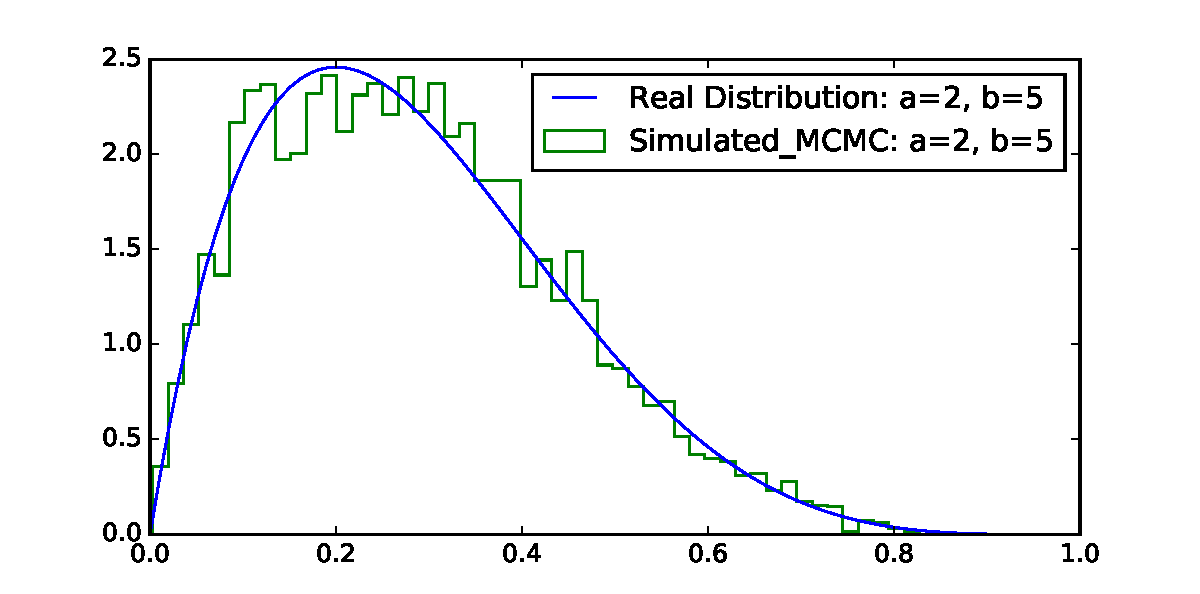
\includegraphics[width = 0.85 \textwidth]{beta.pdf}
	\caption{beta 分布模拟图}
	\label{beta}
\end{figure}

总结一下, 对于分布$p(x)$, 我们构造了转移矩阵$Q'$, 使其满足了细致平稳条件
\begin{equation*}
p(x) Q'(x \rightarrow y) = p(y) Q'(y \rightarrow x)
\end{equation*}

其实, 此处$x$并不要求是一维的, 对于高维空间的$p(\bm{x})$, 如果满足细致平稳条件
\begin{equation*}
p(\bm{x}) Q'(\bm{x} \rightarrow \bm{y}) = p(\bm{y}) Q'(\bm{y} \rightarrow \bm{x})
\end{equation*}

那么以上的 Metropolis-Hastings 算法一样有效.


\subsection{Gibbs Sampling}
假设要从高维分布中进行采样, 样本的联合分布为$p(x_1, x_2, \cdots, x_n)$, 我们要采样得到样本$\bm{X} = (x_1, x_2, \cdots, x_n)$.

对于高维的情形, 由于接受率$\alpha$的存在(通常$\alpha < 1$), 以上 Metropolis-Hastings 算法的效率并不高. 于是有了 Gibbs Sampling.

\begin{algorithm}[htb]
\caption{算法: Gibbs 采样算法}

\begin{enumerate}[1.]
\item  随机初始化$\{ x_i, i = 1, 2, \cdots, n \}$

\item 对$t = 0, 1, 2, \cdots$, 循环从满条件分布中采样
\begin{itemize}
    \item $x_{1}^{(t+1)} \sim p(x_1 | x_{2}^{(t)}, x_{3}^{(t)}, \cdots, x_{n}^{(t)})$
    \item $x_{2}^{(t+1)} \sim p(x_2 | x_{1}^{(t+1)}, x_{3}^{(t)}, \cdots, x_{n}^{(t)})$
    \item $\cdots$
    \item $x_{j}^{(t+1)} \sim p(x_j | x_{1}^{(t+1)}, \cdots, x_{j-1}^{(t+1)}, x_{j+1}^{(t)} ,\cdots, x_{n}^{(t)})$
    \item $\cdots$    
    \item $x_{n}^{(t+1)} \sim p(x_n | x_{1}^{(t+1)}, x_{2}^{(t+1)}, \cdots, x_{n-1}^{(t+1)})$
\end{itemize}
\end{enumerate}

\end{algorithm}



\section{关于 MCMC 的补充}












\section{总结}
\subsection{参考资料}
\begin{enumerate}[(1)]
\item 博客: \url{http://sunyi514.github.io/2016/03/05/mcmc%E6%96%B9%E6%B3%95%E5%B0%8F%E8%AE%B0/?utm_source=tuicool&utm_medium=referral}, 有简单介绍和 Python 编程.

\item 博客: \url{http://www.flickering.cn/%E6%95%B0%E5%AD%A6%E4%B9%8B%E7%BE%8E/2014/06/lda%E6%95%B0%E5%AD%A6%E5%85%AB%E5%8D%A6mcmc-%E5%92%8C-gibbs-sampling/}, 理论介绍的更为详细一些.


\end{enumerate}




\newpage

\section*{附录}








\end{document}